\chapter{Introduction}
This course builds directly on the techniques you may have learned in  MA0232 Modelling with Differential Equations. As in MA0232 we will develop techniques that allow us to model biological phenomena and, in particular, derive properties of the equations without explicitly solving them.

This may seem counter-intuitive as we have a variety of techniques that enable us to solve many of the equations that we see in closed form. Further, numerical simulations can be used to illustrate equations that we cannot solve analytically. However, even when direct solutions are available, they may not always enable clear interpretations and understanding of the underlying system. Equally, our analytical techniques will give us confidence in the solutions produced by numerical software.

Initially, we will focus on systems where the dynamics are spatially homogeneous. In other words the interactions are occurring uniformly across space, the agents we are modelling are `\textit{well mixed}' and we only need to consider the evolution of the agent populations over time. Such dynamics are typically modelled (but not exclusively, as we will see in Chapter \ref{Spatial systems}) using ordinary differential equations, ODEs.

We will then proceed to consider systems where there is explicit spatial variation. In  ecological and biological contexts the main physical phenomenon governing the spatial movement of agents is typically (but again not exclusively),  diffusion. Diffusion, as we will see in Chapter \ref{Spatial systems} models random movement, thus, we are generally assuming that our agents do not have a preferred movement direction.

However, before we investigate such interesting cases as animal pigmentation patterning and neural pulses we must begin at the start with the techniques you should have already covered.

\section{References}
The main references for this lecture course will be:
\begin{itemize}
\item J. D. Murray, Mathematical Biology, 3rd edition, Volume I.
\item J. D. Murray, Mathematical Biology, 3rd edition, Volume II.
\end{itemize}
\begin{figure}[!!!h!!!tb]
\centering
\subfigure[\label{MBI}]{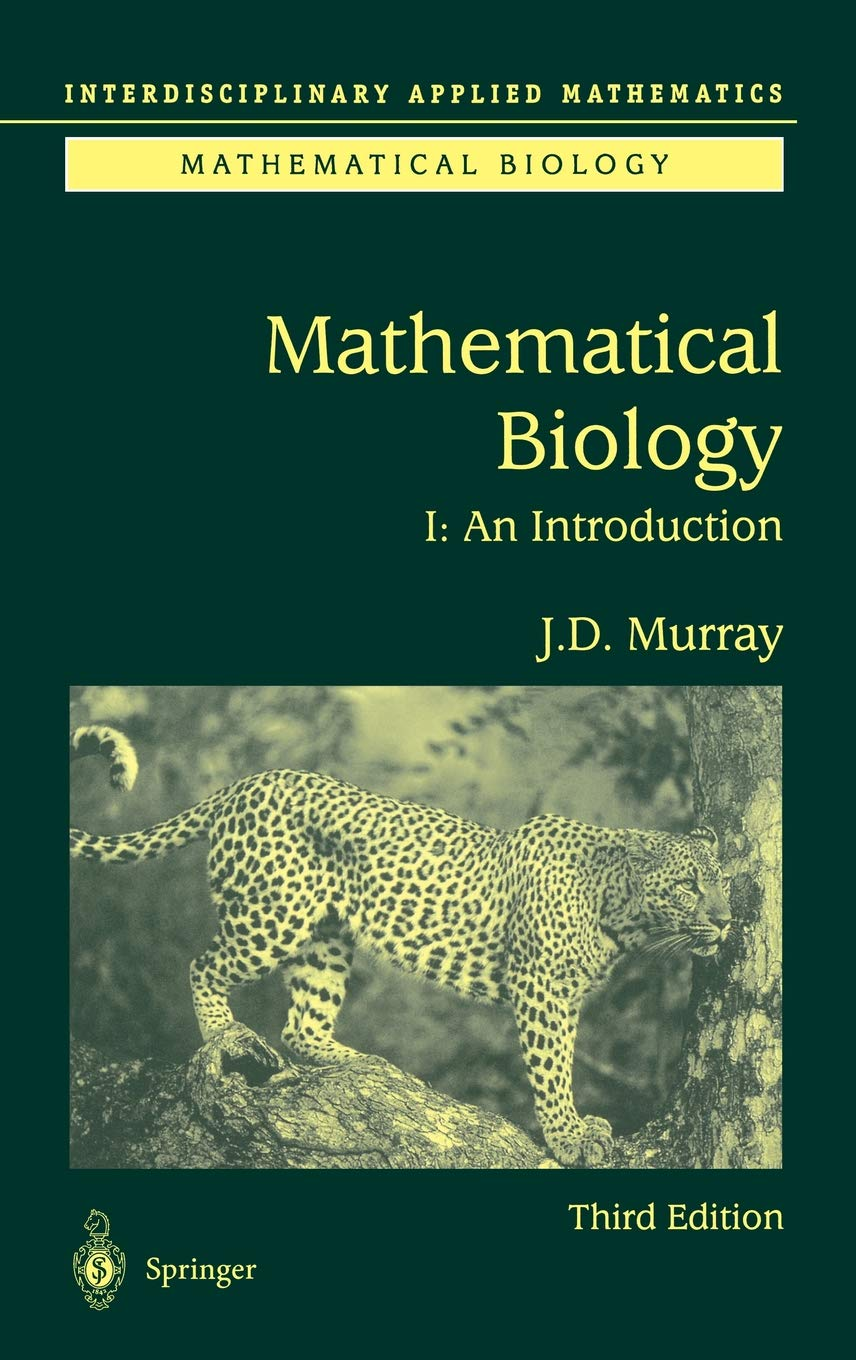
\includegraphics[height=\ttp]{../Pictures/9780387952239.jpg}}
\subfigure[\label{MBII}]{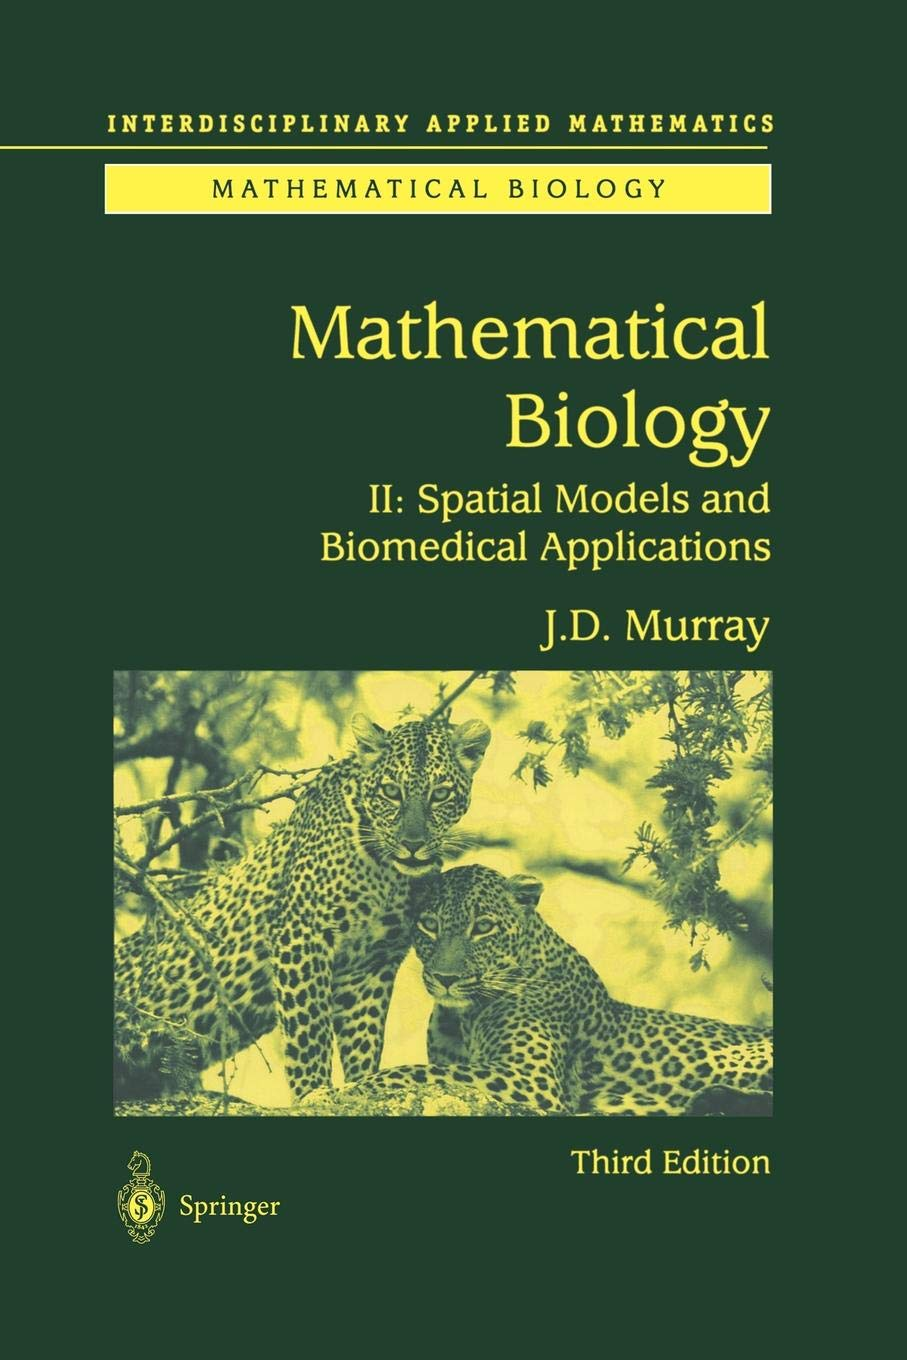
\includegraphics[height=\ttp]{../Pictures/9780387952284.jpg}}
\subfigure[\label{TEWPKMJDM}]{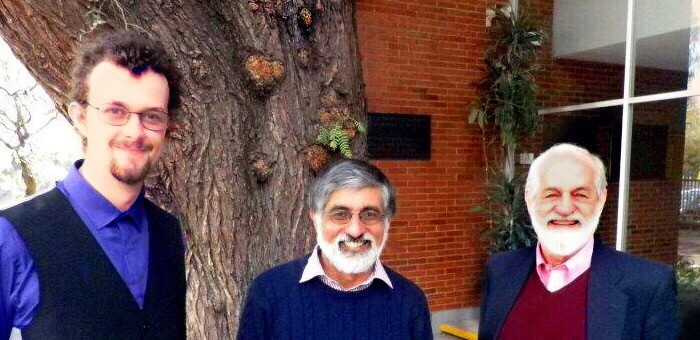
\includegraphics[width=\ttp]{../Pictures/TPJ_cropped2.jpeg}}
\caption{ \label{Books} (a), (b) The bibles of Mathematical Biology. (c) Prof. Jim D. Murray (right), Prof. Philip K. Maini (centre) and Dr Thomas E. Woolley (left).}
\end{figure}
Other useful references include:
\begin{itemize}
\item J. P. Keener and J. Sneyd, Mathematical Physiology.
\item L. Edelstein-Keshet, Mathematical Models in Biology.
\item N. F. Britton, Essential Mathematical Biology.
\end{itemize}
\Chapter{Things you have forgotten}
Whilst we are considering spatially uniform dynamics we will be concerned with ordinary differential equations, ODEs.

\begin{defin}
An ordinary differential equation (ODE) is a differential equation containing one or more functions of \underline{\textbf{exactly one}} independent variable and its derivatives.
\end{defin}

We will be considering the rate of change of a variable, $u$, with respect to another variable, $t$, normally time. This dependence will be denoted
\bb
u(t).
\ee
Here, $u$ is a scalar function (\ie one-dimensional), but more generally, we will be considering systems of variables
\bb
\bm{u}(t)=\l u_1(t),u_2(t),\dots,u_k(t)\r.
\ee
The values of $u$ or $\bm{u}$ define quantities of interest. For example they could be an animal population density, or biochemical concentrations. On the board we will usually write bold symbols with an underline\footnote{I was once told that we use underlines to illustrate bold variables because when typesetting a document an underline would tell the printer that that symbol needed to be bold. However, if this is true, how did the writer indicate that they wanted a symbol underlined?} as it is easier to see, thus, $\bm{u}=\underline{u}$.


In order to link the changes in these quantities we define a system of ODEs in the most general way possible,
\bb
\bm{F}\l t,\bm{u},\frac{\rd \bm{u}}{\rd t},\frac{\rd^2 \bm{u}}{\rd t^2},\dots,\frac{\rd^n \bm{u}}{\rd t^n}\r=0,
\ee
with initial condition given by
\bb
\bm{u}(0)=\bm{u}_0.
\ee
Note that the initial condition is kept general as we will usually be interested in how the dynamics of the system change for different starting points.

\begin{defin}
A system of differential equations is \textbf{autonomous} if the system does not explicitly depend on the independent variable.
\end{defin}
When the variable is time, they are also called time-invariant systems, this simply means that we are assuming that the defined underlying laws of the system are identical to those for any point in the past, or future.

\begin{defin}
To save time we use a dot or prime mark to denote a derivative with respect to the argument, thus,
\bb
\dot{\bm{u}}(t)=\bm{u}'(t)=\frac{\rd \bm{u}}{\rd t}.
\ee
\end{defin}
Traditionally, dots are primarily used when the variable is time and primes are used otherwise. Note that higher orders derivatives are signified by the appropriate number of dots or primes. Namely, a second derivative would be denoted by two dots or primes, etc.

In this course we are going to occupy ourselves with systems of autonomous first order equations, of the form
\bb
\frac{\rd \bm{u}}{\rd t}=\dot{\bm{u}}=\bm{F}(\bm{u}).\label{ODE}
\ee
This may seem highly restrictive. However, systems of first order equations can have extremely complicated properties, such as oscillations and chaos, which we will try to understand.

\section{How to model a system}\label{How to model a system}
Modelling a system, whether it be physical, chemical, or biological, is, in some ways, more of an art than a science. You try and strip away all extraneous information and mathematically describe that which is left. In physics there are physical laws to help you, \eg gravity, conservation of energy and mass. Unfortunately, biology has no such fundamental laws. Thus, we must use experimental intuition, \eg predator-prey interactions from population data. Critically, the modelling should always form part of a cyclical process \see{Modelling_loop}.

You try to start with physical intuition (experiment), represent the important parts mathematically (model), hopefully reproduce reality (test) and, finally, use your mathematical model to predict unknown outcomes (predict). These predictions can then feed back into experiment and the process begins anew.
\begin{figure}[!!!h!!!tb]
\centering
\includegraphics[width=\tp]{../Pictures/Modelling_loop.png}
\caption{\label{Modelling_loop}Diagram of the modelling cycle.}
\end{figure}

\section{Law of Mass Action}
In this section we will learn about a very general technique that will allow us to build an ODE system out of multiple interacting populations. These populations could represent chemical compounds, humans, cells or animals as well as different states within a population \ie infected humans and susceptible humans. The law presented in this section is applied whenever the populations of the system are able to: (i) change identities; (ii) create more population members; or (iii) cause populations to decay. Specific examples of each of these interactions are, respectively: (i) susceptible humans becoming infected through interactions with a diseased person; (ii) animals giving birth; (iii) predators eating prey. Note that a change-of-identity interaction can itself be thought as a combination of creation and degradation operations. For example, in the above case of infection a member of the susceptible human population is removed from the system, whilst an infected human is added to the system. Thus, all interactions can be made through combining creation and degradation operations.

We use chemical reaction notation to specify the outcomes of population interactions. Consider a system composed of $n$ different interacting populations $(u_1,\dots,u_n)$. We assume that all interactions between the population elements lead to the creation, or destruction, of one (or more) of the $n$ populations. 
\begin{defin}
A \textbf{rate equation} specifies that an interaction involves $a_1$ members of population $u_1$, $a_2$ members of population $u_2$, etc. and produces $b_1$ members of population $u_1$, $b_2$ members of population $u_2$, etc. The equation is written as
\bb
a_1u_1+a_2u_2+\dots+a_nu_n \stackrel{r}{\rightarrow} b_1u_1+b_2u_2+\dots+b_nu_n,
\ee
where $r>0$ is the \textbf{reaction rate}.
\end{defin}
Note that some of the $a_i$ and $b_i$ values can be zero.



Rate equations provide a rigorous way of defining all of the interactions a system is assumed to undergo. However, we still require a method of converting the rate equation into an ODE. This is the power of the Law of Mass Action.
\begin{defin}
The \textbf{Law of Mass Action} states that production rate of a reaction is directly proportional to the product of the input population sizes. Specifically, if 
\bb
a_1u_1+a_2u_2+\dots+a_nu_n \stackrel{r}{\rightarrow} b_1u_1+b_2u_2+\dots+b_nu_n \nonumber
\ee
is the reaction of interest then the production rate is proportional to
\bb
ru_1^{a_1}u_2^{a_2}\dots u_n^{a_n}
\ee
and the accompanying ODEs are
\begin{align}
&\dot{u}_1=(b_1-a_1)ru_1^{a_1}u_2^{a_2}\dots u_n^{a_n},\\
&\dot{u}_2=(b_2-a_2)ru_1^{a_1}u_2^{a_2}\dots u_n^{a_n},\\
&\vdots\\
&\dot{u}_n=(b_n-a_n)ru_1^{a_1}u_2^{a_2}\dots u_n^{a_n}.
\end{align}
\end{defin}
Note that in converting from reaction equation to the ODE of $u_i$ we to account for the stoichiometry, \ie $(a_i-b_i)$. Further, when multiple reactions are considered, the terms arising from the Law of Mass Action are simply added together as independent terms.

\begin{example}[frametitle=Creating logistic growth]\label{Reaction equation examples}
Consider a bacterial population $u$ and a nutrient population $v$, such that the bacteria uses the nutrient to reproduce, \ie,
\bb
u+v\stackrel{R}{\rightarrow}2u,\nonumber\\
\ee
and the initial conditions are $u(0)=u_0$ and $v(0)=v_0$.

\COL{
Using the Law of Mass Action we derive the following two equations:
\begin{align}
&\dot{u}=Ruv,\label{Logistic_u}\\
&\dot{v}=-Ruv.
\end{align}
Adding the equations together we find that 
\bb
\frac{d}{dt}(u+v)=0,
\ee
meaning that $u+v=$ constant $=u_0+v_0=K$ for all time. We can substitute this formula into \eqn{Logistic_u} to get
\bb
\dot{u}=Ru(K-u)=RKu\l 1-\frac{u}{K}\r =r u\l 1-\frac{u}{K}\r,\label{Logistic_equation}
\ee
where we have defined a new parameter $r=RK$, known as the growth rate and $K$ is know as the carrying capacity. Overall, \eqn{Logistic_equation} is known as the logistic equation.
}
\end{example}





\section{Non-dimensionalisation}\label{Non-dimensionalisation}
To non-dimensionalise a system of equations, we have the following rules:
\begin{enumerate}
\item Identify all the variables;
\item Replace each variable with a quantity scaled relative to a characteristic unit of measure (to be determined);
\item Choose the definition of the characteristic unit for each variable;\label{Choose}
\item Rewrite the system of equations in terms of the new dimensionless quantities.
\end{enumerate}
We note three particular points about these rules. Firstly, the theory behind non-dimensionalisation is straight forward. Namely, we substitute scaled variables into an equation system and massage the equations until we have rearranged the system to produce the desired outcome. However, in practice the difficulty of the technique lies in the algebraic manipulation; it is very easy for the terms to become lost during the manipulation. Thus, care must be taken during the algebraic manipulation stage.

Secondly, you will notice the word `choose' in point \ref{Choose}. This means that it possible to construct many different non-dimensionalised systems from the same system of equations, \ie non-dimensionalisation is non-unique. We usually choose the characteristic unit of each variable to either emphasise one of the terms in a system or to remove as many parameters as possible.

Finally, this technique is hard to demonstrate in generality. It is much better to consider a number of examples and see how the technique works in action. Thus, what follows will be a select number of examples, which along with your problem sheets should give you a good basis in the theory. However, do not think that these are all the examples you could face.

It should be noted that there is little consistency in nomenclature across book when considering the separation of variables into their dimensional and non-dimensional components. Thus, always be clear in your definitions.

\subsection{Examples of non-dimensionalisation through substitution of variables}\label{Examples of non-dimensionalisation through substitution of variables}
\begin{example}[frametitle=Substituting variables]
Consider the equation for logistic growth,
\bb
\dot{u}=ru\l 1-\frac{u}{K} \r, \quad u(0)=u_0.\label{Non-dim_2}
\ee
\COL{Again, $u=[u]u'$ and $t= [t]t'$ can be substituted into \eqn{Non-dim_2} to produce
\bb
\frac{\rd u'}{\rd t'}=[t]ru'\l 1-\frac{[u]}{K}u'\r,\quad u'(0)=\frac{u_0}{[u]},\nonumber
\ee
from which we see that it would be wise to take $[t]=1/r$. Beyond this we see that we have a choice. Should we take $[u]=K$, or $[u]=u_0$? Both are valid non-dimensionalisations and either maybe be appropriate depending on the context of the problem. 

Here, we are going to take $[u]=K$ as we are interested in the dynamics of the system, rather than the initial condition. Thus, after dropping primes, for notational convenience, we see that we can non-dimensionalise \eqn{Non-dim_2} to 
\bb
\frac{\rd u}{\rd t}=u\l 1-u\r,\quad u(0)=U_0,\nonumber
\ee
where $U_0=u_0/[u]=u_0/K$. 

For mathematicians dropping primes is often done as the last step because we infrequently care about the actual values of the variables, rather we study the dynamics available in the equation. However, in any specific application we should be careful to remember that the variables we are dealing with are non-dimensional and that the solution is not complete until we `re-dimensionalise' the variables.

In this case the non-dimensionalisation demonstrates that the only parameter that the solution depends on is the initial conditions. Changing $r$ does not change the dynamics of the system, it only changes the time scale, since $r=1/[t]$. Equally, changing $K$ simply scales the size of the solution, as $u=Ku'$.}
\end{example}

\subsection{Examples of non-dimensionalisation through the arrow method}
The substitution method shown in \sect{Examples of non-dimensionalisation through substitution of variables} will always work, assuming that the algebra is manipulated correctly. However, the method can be cumbersome and slow. Moreover, because it involves lots of algebraic manipulations there are many chances to make a mistake.

An alternative method rests on using arrows to identify the desired balances. This can be much quicker as the initial stages do not require laborious substitution. However, we have to be more careful because not all balances that we can `draw' using the arrows will be valid.

The idea behind the arrow method is that you draw arrows between the quantities that are going to `balance', which simply means they are going to have the same coefficient in the final non-dimensionalised form. The process is generally the same as the substitution method. However, we must remember that in order to specify the problem completely the number of valid arrow balances must equal the number of variables. For example, if a problem depends on $u$ and $t$ we would need two balances. Alternatively, if the problem depended on $u$, $v$, and $t$ we would need three valid balances.
\begin{example}[frametitle=Arrow method]\label{Arrow method}
\item Consider the following equation
\bb
  \tikzmark{a}\dot{u}=k_0+k_1\tikzmark{b}u+k_2\tikzmark{c}u^2, \quad u(0)=u_0.\label{Non-dim_4}
\tikz[overlay,remember picture]
{\draw[square arrow1] (a.south) to (b.south);}
\tikz[overlay,remember picture]
{\draw[square arrow1] (b.south) to (c.south);}
\ee
\COL{We have two variables, $u$ and $t$, and so we need two balances. Specifically, the arrows state that we want to balance the derivative, linear and quadratic terms,
\bb
\frac{[u]}{[t]}=k_1[u]=k_2[u]^2,\nonumber
\ee
from which it is simple to discover that
\bb
[t]=\frac{1}{k_1},\quad [u]=\frac{k_1}{k_2}.\nonumber
\ee
We still need to substitute the scales into the equations. Namely, $u=u'k_1/k_2$ and $t=t'/k_1$, but again the arrow method simplifies this task. Specifically, we know that, by design, the coefficient of the derivative, linear and quadratic term are going to be the same. Thus, we can divide through by one of them to speed up the derivation,
\bb
\frac{\rd u'}{\rd t'}=\frac{k_0}{k_1[u]}+u'+u'^2.\nonumber
\ee
Finally, redefining the last parameter as $\alpha=k_0/(k_1[u])=k_0k_2/(k_1^2)$ and the initial condition $u'(0)=k_2u_0/k_1=u'_0$, we can non-dimensionalise \eqn{Non-dim_4} to the final form of
\bb
\dot{u}=\alpha+u+u^2,\quad u(0)=u'_0,\label{Non-dim_5}
\ee
where we have dropped the primes from the variables for simplicity.}

\end{example}



\section{Stationary states and stability}\label{Stationary states and stability}
Now that we are able to model and simplify a physical system, we want to predict what the equations will do without having to simulate the system each time. Specifically, we are not interested in the transient initial behaviour of the equations, we want to understand what the trajectories will like look far into the future. To enable us to generate insights we first need two important definitions.
\begin{defin}
A state, $\bm{u}_s$, is a \textbf{steady state} or \textbf{stationary state} of the ODE system
\bb
\dot{\bm{u}}=\bm{F}(\bm{u})
\ee
if it satisfies $\bm{F}(\bm{u}_s)=0$.
\end{defin}
This definition simply states that if the ODE system ever reaches $\bm{u}_s$ then the system will not evolve further because all of the dynamics are in equilibrium. This is a useful concept, but currently incomplete.

For example, you can (theoretically) stand a pencil on its tip and it would remain stationary, if it were not perturbed \see{Pencil_stationary_state}. Hence, this is a stationary state orientation of the pencil. However, it would require only a very small perturbation to cause the pencil to fall over and, thus, transition from the state of being on its point to being on its side \see{Pencil_stationary_state}. Given a large enough perturbation (\ie picking the pencil up) you could reset the pencil to the previous state of standing on its point. However, it requires a larger perturbation to reset the pencil than it does to knock it over and, so, we see that although these state are both stationary states they are somehow fundamentally different. This difference comes down to the intuitive concept of `stability'.
\begin{figure}[!!!h!!!tb]
\centering
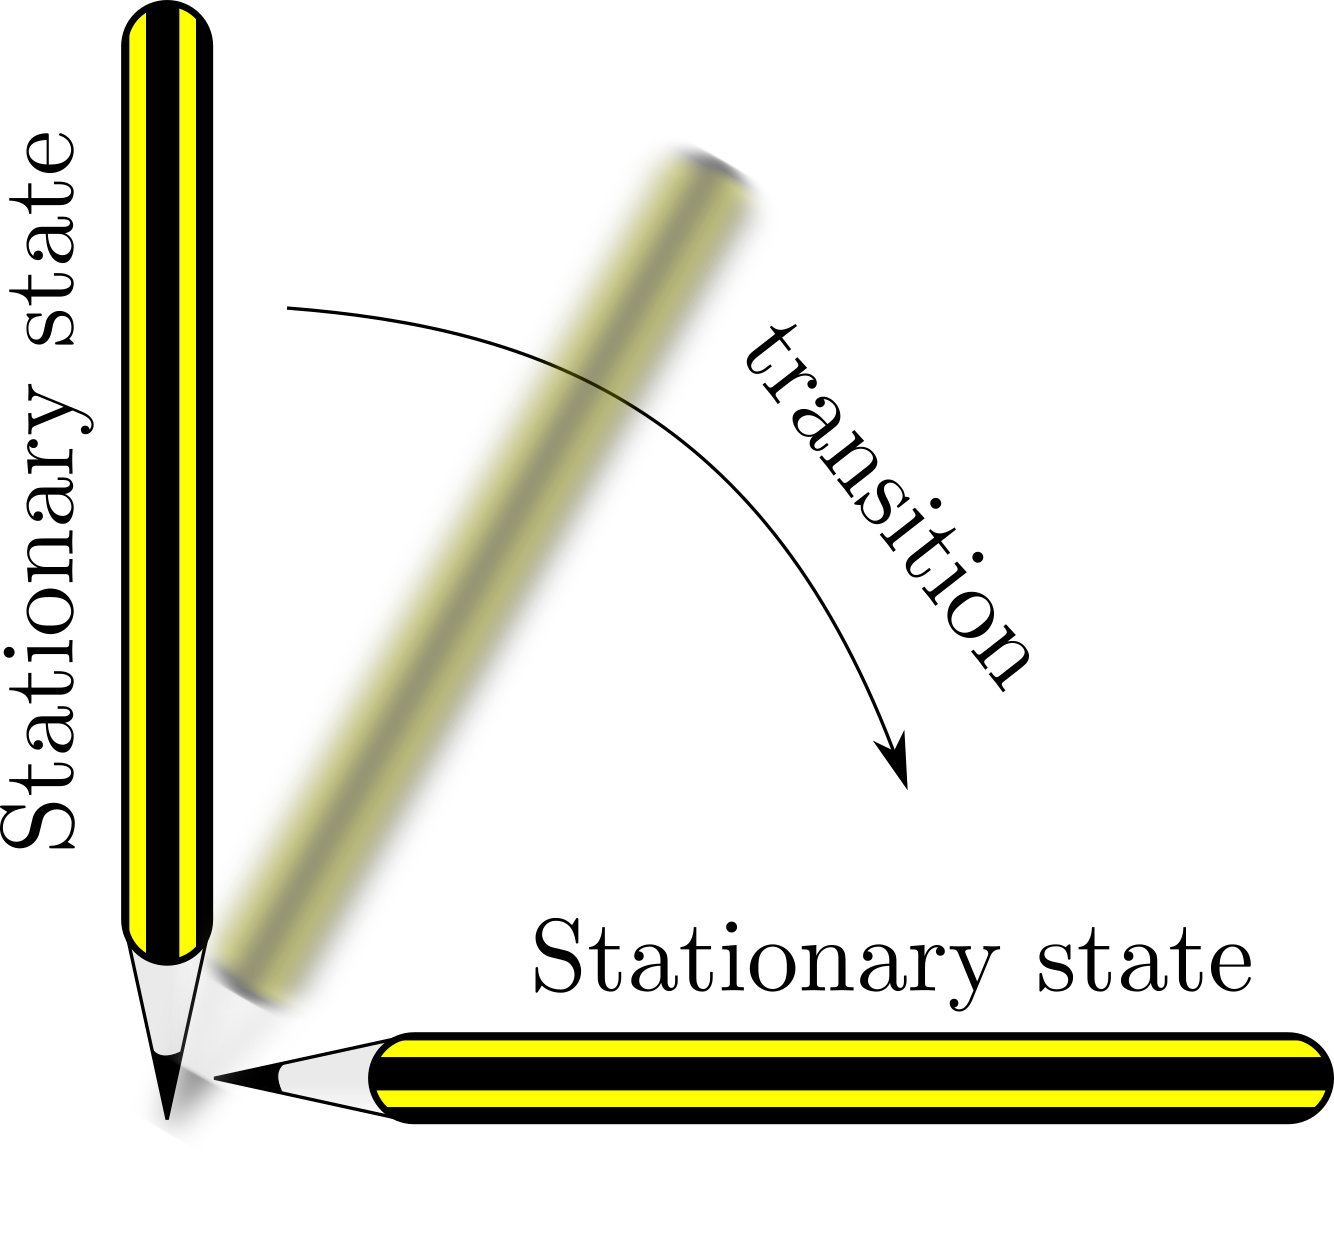
\includegraphics[width=\ttp]{../Pictures/Pencil_stationary_state.png}
\caption{\label{Pencil_stationary_state} Stationary states of a pencil.}
\end{figure}

\begin{defin}
A steady state, $\bm{u}_s$, of the ODE system
\bb
\dot{\bm{u}}=\bm{F}(\bm{u})
\ee
is \textbf{stable} if for all $\epsilon >0$, there exists a $\delta > 0$ and a $t_0>0$ such that whenever $|\bm{u}(t)-\bm{u}_s|< \delta$ then $|\bm{u}(t)-\bm{u}_s|<\epsilon$ for all $t \ge t_0$. Otherwise the steady state is unstable
\end{defin}
Simply put, this means that a state, $\bm{u}_s$, is stable if whenever a solution $\bm{u}(t)$ comes close enough to it then the solution tends to the state \ie $\bm{u}(t)\rightarrow\bm{u}_s$. In the example of the pencil, both the vertical and horizontal orientations of the pencil are stationary states. However, only the horizontal orientation is stable.



\section{Linear stability}
Having a definition of stability is one thing, but we need a method of characterising whether a system is stable or unstable. The crux of this characterisation is to consider the dynamics of an ODE system near its stationary points. To do this we substitute a solution into the equations that is a perturbation about the steady state. Using Taylor series we expand the system in terms of the perturbation and keep only the linear terms as we are assuming that the perturbation is small. Since the system is now linear we can solve the approximate equations completely and, thus, they will tell us what dynamics to expect close to the steady states.
\begin{thm}\label{Stability_theorem}
Suppose $u_s$ is a steady state of the one dimensional ODE,
\bb
\dot{u}=F(u),\label{General_ODE}
\ee
then $u_s$ is linearly stable if $\rd F(u_s)/\rd u<0$ and linearly unstable if $\rd F(u_s)/\rd u>0$.
\end{thm}
\begin{proof}
The proof can be found in \app{Proof of stability criterion for scalar ODE equations}.
\end{proof}
We make a number of remarks about the theorem's statement:
\begin{itemize}
\item The theorem makes no claim about the solutions properties in the case that the first derivative $\rd F(u_s)/\rd u=0$. In this specific case we would have to go to higher order in the Taylor expansion.
\item Linear stability only tells us what happens close to the steady state. Thus, although a state may be stable, we have no metric for how close we have to be to the steady state before we are attracted to the stable point.
\item In the case that $u_s$ is unstable we cannot conclude what happens to the trajectory. Indeed, a trajectory near an unstable point may grow without bound or, simply tend to one of the other stationary states in the system that is stable.
\end{itemize}
\begin{example}[frametitle=Stationary states and stability of the logistic equation\label{Logistic_stability_example}]
The non-dimensionalised logistic equation is (as we have seen before)
\bb
\dot{u}=u(1-u).\label{Logistic_stability}
\ee
\COL{Firstly, we calculate the steady states by setting $\dot{u}=0$. Trivially, we can see that the steady }\COL{are $u=0$ and $1$. Next we calculate the derivative of the right-hand side of \eqn{Logistic_stability} with respect to $u$,
\bb
F(u)=u(1-u) \implies F'(u)=1-2u.
\ee
Since,
\begin{align}
&F'(0)=1>0,
&F'(1)=-1<0,
\end{align}
then, from Theorem \ref{Stability_theorem}, we deduce that 0 is an unstable steady state and 1 is a stable steady state. These results are confirmed in \fig{Logistic_multi_IC}.}
\end{example}
\begin{figure}[!!!h!!!tb]
\centering
\includegraphics[width=\ttp]{../Pictures/Logistic_multi_IC.png}
\caption{ \label{Logistic_multi_IC} Multiple simulations of \eqn{Logistic_stability} with different initial conditions, $u_0$, (noted in the legend), illustrating the stationary states and  their stability characteristics.}
\end{figure}


In the case that we have a system of ODEs, we note that the definition of a steady state immediately generalises to any number of variables. Specifically, if we have $n$ variables, $\bm{u}=(u_1,\dots,u_n)$ then there must be $n$ ODEs, $\bm{F}(\bm{u})=(F_1(u_1,\dots,u_n),\dots,F_n(u_1,\dots,u_n))$, one for each variable, in order for the system to be uniquely defined. Thus, the steady states, $\bm{u}_s$, are found from solving $\bm{F}(\bm{u}_s)=0$. The derivation of linear stability also extends to higher similarly, however, we need to first define the Jacobian.
\begin{defin}
The Jacobian, $\bm{J}$, of an ODE system,
\bb
\dot{\bm{u}}=\bm{F}(\bm{u}),
\ee
is the matrix of partial derivatives of each function, with respect to each argument,
\bb
\bm{J}=\left[ \D{F_i}{u_j}\right]_{i,j=1,\dots,n}= \left[ \begin {array}{cccc} \D{F_1}{u_1}&\D{F_1}{u_2}&\dots&\D{F_1}{u_n}\\
\noalign{\medskip}\D{F_2}{u_1}&\D{F_2}{u_2}&\dots&\D{F_2}{u_n}\\
\noalign{\medskip}\vdots&\ddots&\ddots&\vdots\\
\noalign{\medskip}\D{F_n}{u_1}&\D{F_n}{u_2}&\dots&\D{F_n}{u_n}
\end {array} \right]. 
\ee
\end{defin}
For brevity, it is common practice to write a partial derivative as a subscript, \ie
\bb
\D{F}{u}=F_u.
\ee
Equally, unless otherwise specified, we assume that the Jacobian is evaluated at the steady state.

\begin{thm}\label{System_stability}
Suppose $\bm{u}_s$ is a steady state of the ODE system
\bb
\dot{\bm{u}}=\bm{F}(\bm{u}),\label{Vec_ODE}
\ee
where $\bm{F}$ is continuously differentiable everywhere in all of its arguments and the Jacobian is locally invertible. The linear stability of $\bm{u}_s$ will depend on the eigenvalues of the Jacobian. Namely:
\begin{itemize}
\item if all eigenvalues have negative real part then the steady state is stable;
\item if any eigenvalue has positive real part then the steady state is unstable.
\end{itemize} 

In systems of two species we can be more specific and split the cases up further. Namely, suppose the steady state has eigenvalues $\lambda_1$ and $\lambda_2$,
\begin{table}[h!!!]
\resizebox{\textwidth}{!}{%
\begin{tabular}{cc|c}
                                                    & \textbf{Eigenvalue characteristic} & \textbf{Steady state characteristic} \\\hline
\multirow{3}{*}{\textbf{Eigenvalues are real}}      & $\lambda_1 \geq \lambda_2>0$       & Unstable node                        \\
 & $\lambda_1>0>\lambda_2$      & Saddle point  \\
 & $0>\lambda_1\geq\lambda_2$   & Stable node   \\\hline
\multirow{3}{*}{\textbf{Eigenvalues are imaginary}} & $\textrm{Re}(\lambda_1) \geq \textrm{Re}(\lambda_2)>0$       & Unstable spiral                      \\
 & $\textrm{Re}(\lambda_1) = \textrm{Re}(\lambda_2)=0$    & Centre node   \\
 & $\textrm{Re}(\lambda_1) \leq \textrm{Re}(\lambda_2)<0$ & Stable spiral
\end{tabular}%
}
\end{table}\end{thm}
\begin{proof}
The proofs for general systems can be found in \app{Proof of stability criterion for ODE systems} and the specific proof for two species systems can be found in \app{Characterising the stability of a two-dimensional ODE system}.
\end{proof}

\begin{defin}
A bifurcation point of a system is a parameter value at which the characteristics of the steady states change. This can be either in number of steady states, or their stability.
\end{defin}

\begin{example}[frametitle=Schnakenberg kinetics\label{Schnakenberg_kinetics}]
Calculate the steady state of the following system of equations
\begin{align}
&\dot{u}=f(u,v)=-u+u^2v,\\
&\dot{v}=g(u,v)=\beta-u^2v,
\end{align}
and characterise its stability.

\COL{The steady state, $(u_s,v_s)$, satisfies
\begin{align}
&0=f(u,v)=-u_s+u_s^2v_s,\label{Schnak_1}\\
&0=g(u,v)=\beta-u_s^2v_s.\label{Schnak_2}
\end{align}
Adding \eqns{Schnak_1}{Schnak_2} together we get that $u_s=\beta$ and, thus, from \eqn{Schnak_2} $v_s=1/\beta$. The Jacobian at the steady state is
\bb
J=\left[ \begin{array}{cc}\noalign{\medskip} -1+2u_sv_s&u_s^2\\
-2u_sv_s&-u_s^2
\end {array} \right]=\left[ \begin{array}{cc}\noalign{\medskip} 1&\beta^2\\
-2&-\beta^2
\end {array} \right].
\ee
The eigenvalues, $\lambda$, satisfy
\bb
0=(1-\lambda)\l -\beta^2 -\lambda\r+2\beta^2 =\lambda^2-\lambda\l 1-\beta^2\r+\beta^2,
\ee
and, so,
\bb
2\lambda_\pm=1-\beta^2\pm\sqrt{(1-\beta^2)^2-4\beta^2}.\label{Schnak_lam}
\ee
From \eqn{Schnak_lam} we notice that $\lambda_{\pm}>0$ whenever $\beta^2<1 \implies 0<\beta<1$ and that $\lambda_\pm$ are complex when,
\begin{align}
(1-\beta^2)^2-4\beta^2<&0,\nonumber\\
\implies-2\beta<(1-\beta^2)<&2\beta,\nonumber\\
\implies\beta^2-2\beta-1<0<&\beta^2+2\beta-1,\nonumber\\
\implies -1+\sqrt{2}<\beta<&1+\sqrt{2}.\nonumber
\end{align}}
\end{example}
\begin{figure}[!!!h!!!tb]
\centering
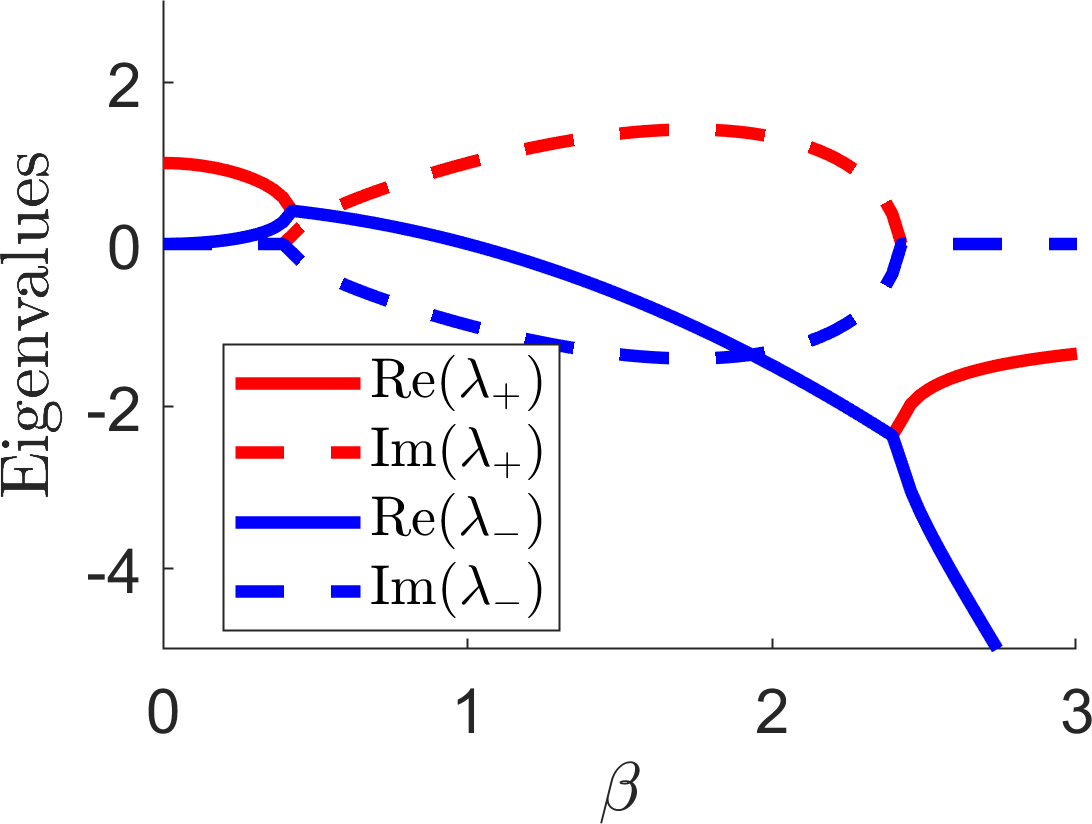
\includegraphics[height=\ttp]{../Pictures/Schnakenberg_stability.png}
\caption{ \label{Schnakenberg_eigenvalues}Plotting the eigenvalues from example \ref{Schnakenberg_kinetics}.}
\end{figure}

\begin{figure}[p!!!h!!!tb]
\centering
\subfigure[\label{beta_0.25}$\beta=0.25$]{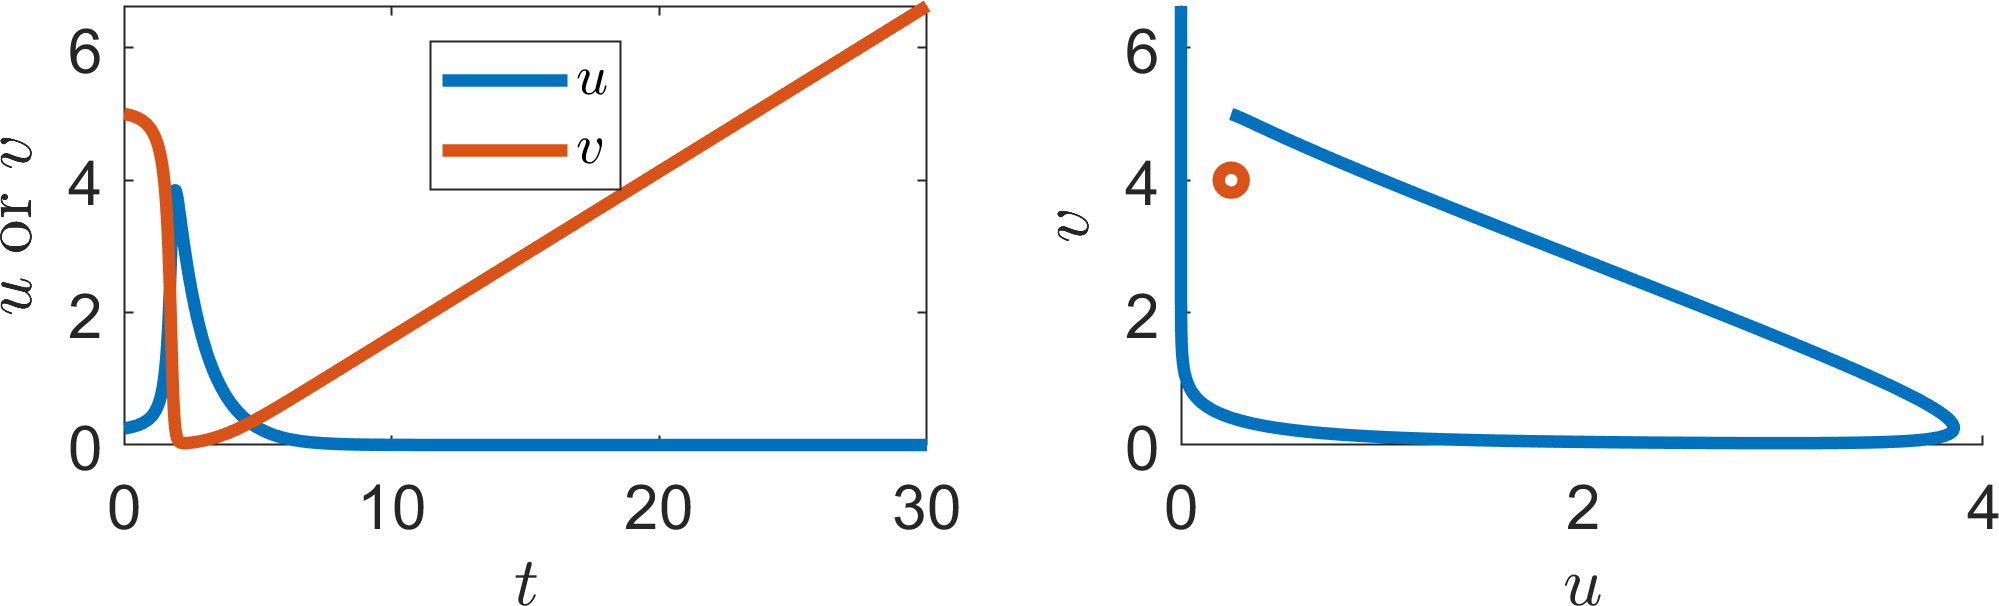
\includegraphics[height=\tttttp]{../Pictures/Schnakenberg_beta_25.png}}
\subfigure[\label{beta_0.75}$\beta=0.75$]{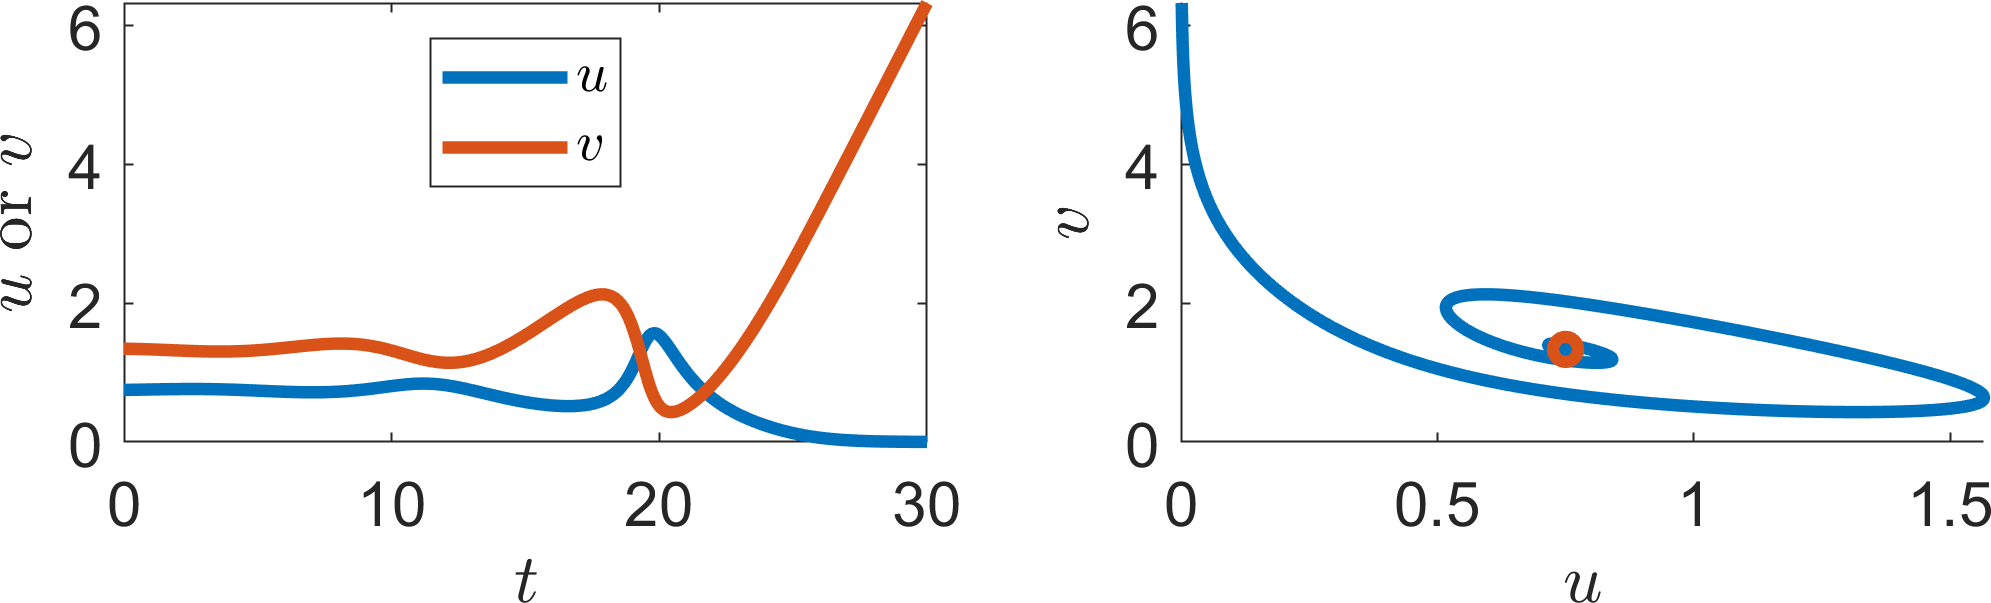
\includegraphics[height=\tttttp]{../Pictures/Schnakenberg_beta_75.png}}
\subfigure[\label{beta_1}$\beta=1$]{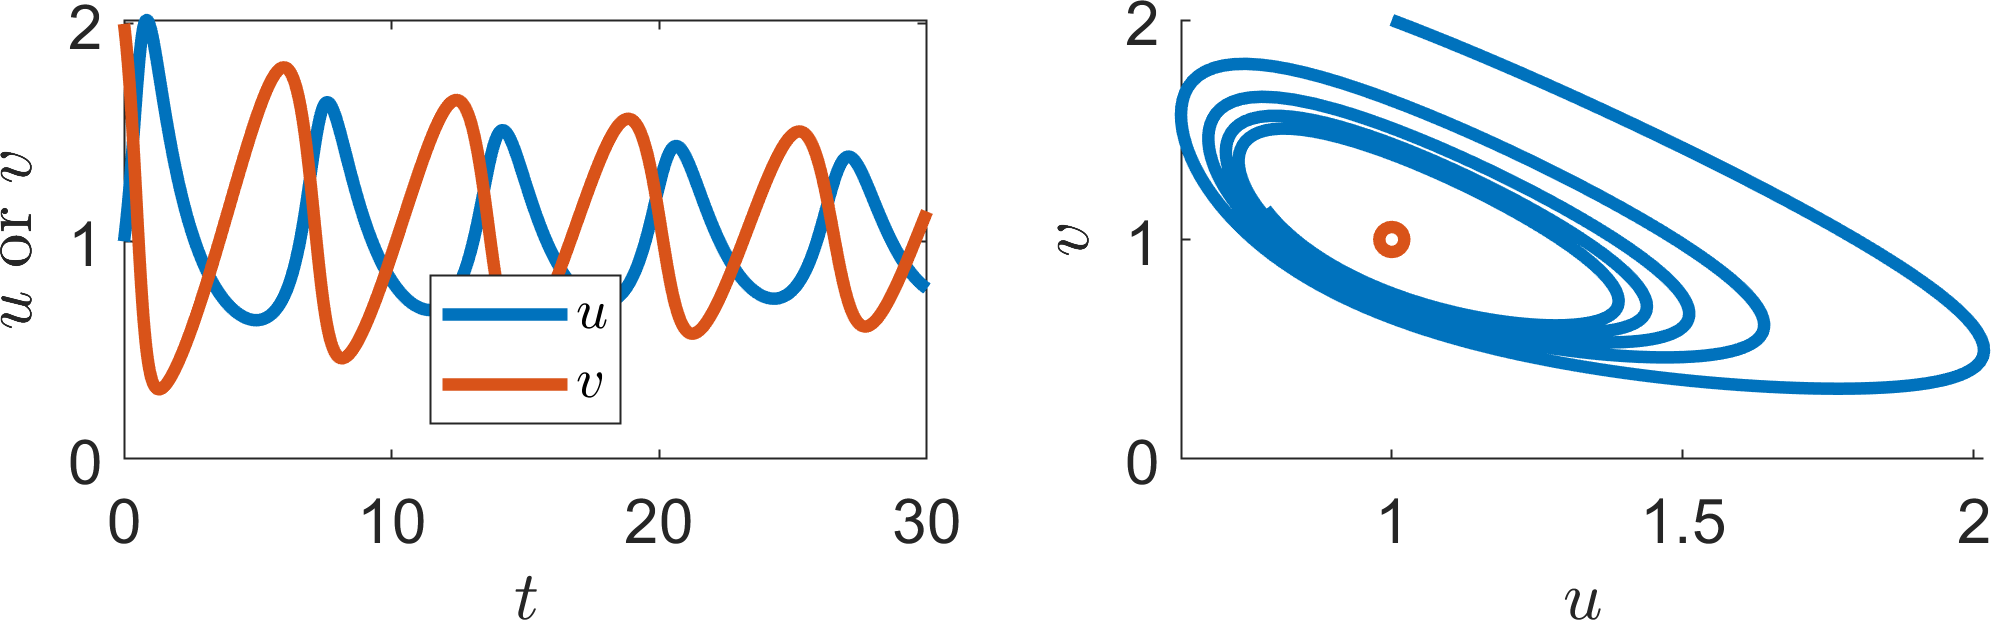
\includegraphics[height=\tttttp]{../Pictures/Schnakenberg_beta_100.png}}
\subfigure[\label{beta_1.2}$\beta=1.2$]{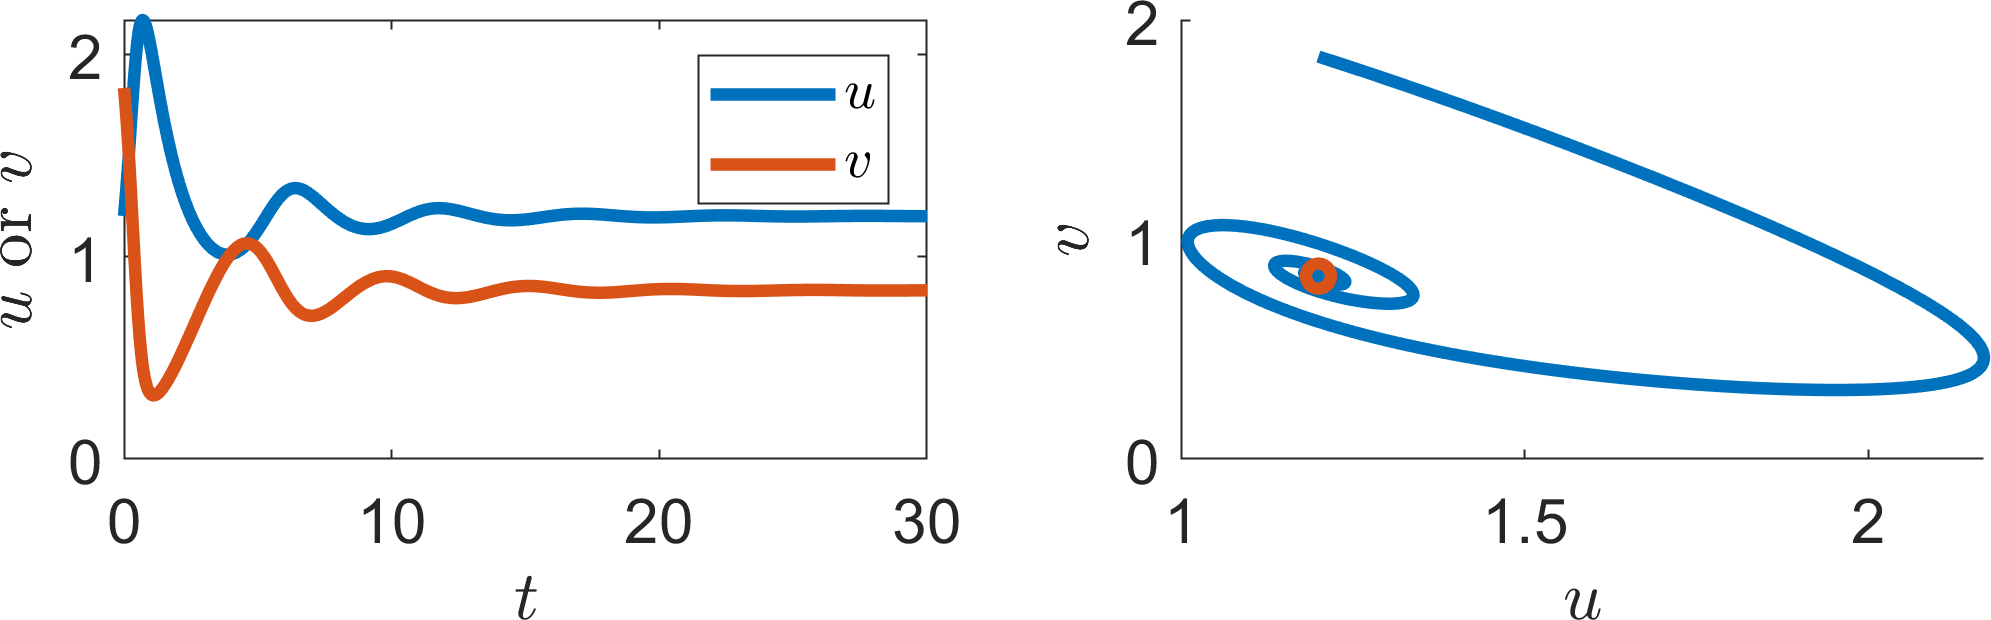
\includegraphics[height=\tttttp]{../Pictures/Schnakenberg_beta_120.png}}
\subfigure[\label{beta_2.5}$\beta=2.5$]{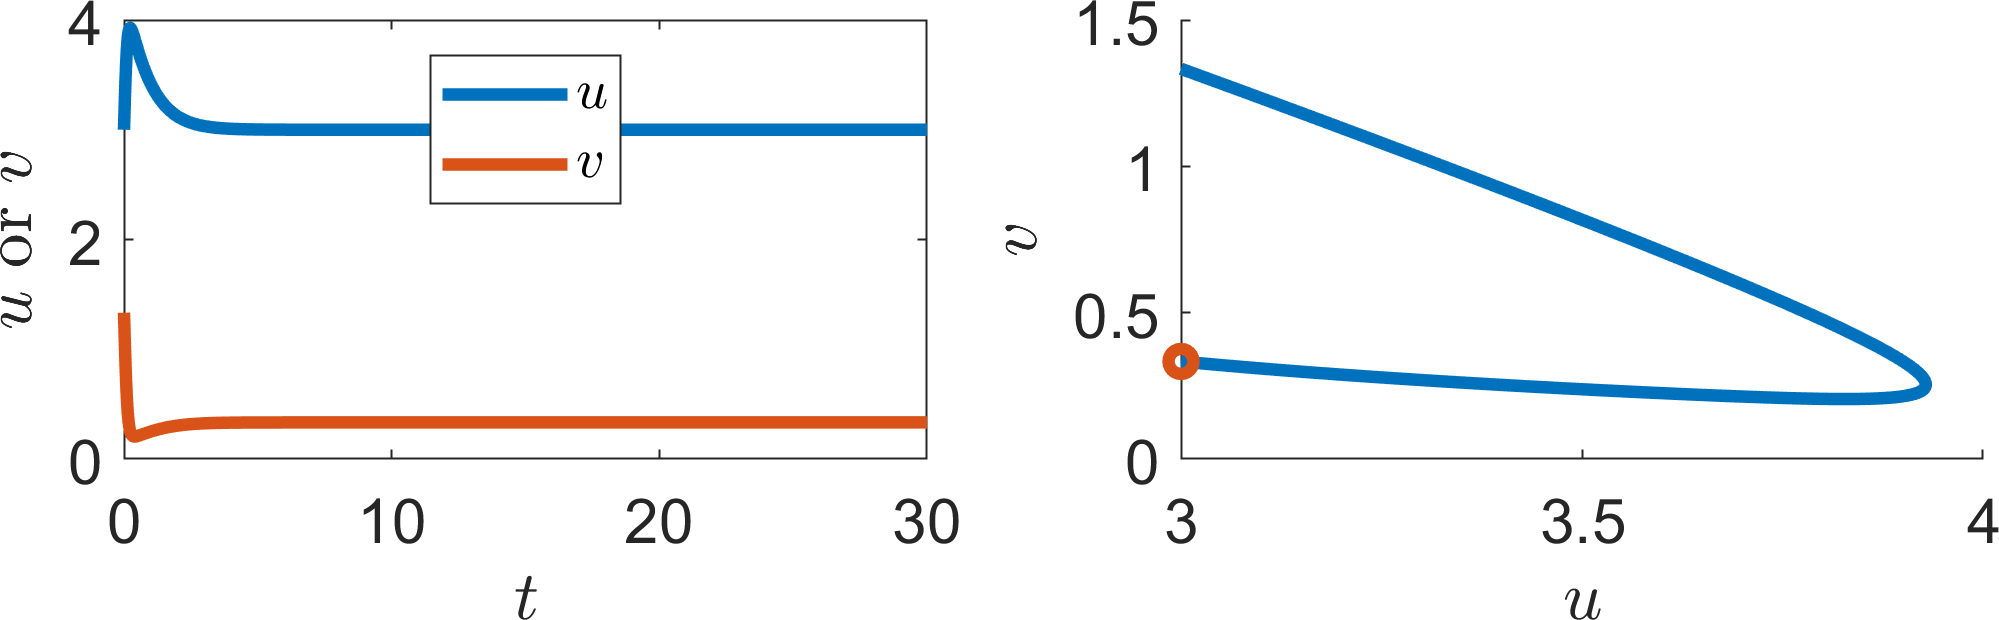
\includegraphics[height=\tttttp]{../Pictures/Schnakenberg_beta_300.png}}
\caption{ \label{Schnakenberg_betas}Illustrating the stationary states and stability characteristics of the Schnakenberg equations from example \ref{Schnakenberg_kinetics}. The left plots show the trajectories of each population over time. The right plots show the corresponding phase planes. The red circle in each case is the steady state $(\beta,1/\beta)$, where $\beta$ is noted beneath each figure.}
\end{figure}


\section{Curve sketching}
Algebraic and analytical solutions will always be the surest way of providing an answer, as they provide all information regarding the quantitative values and parameter dependencies. However, such solutions are not always possible. Sometimes they algebra is not tractable, or the solution might be too cumbersome to provide clear insight. Thus, we often fall back on the skill of curve sketching.

There is no defined process to curve sketching. Essentially, you are looking for simple features that you understand and, thus, the best approach to curve sketching is through gaining experience. Namely, the more functions you sketch the larger your catalogue of known shapes. However, there are some general tips that will help you sketch simple curves, as well as a number of stereotypical examples you should know well.

Suppose we want to sketch the curve $f(x,\mu)$, where $x$ is the argument and $\mu$ is a parameter, the general tips are:
\begin{itemize}
\item look for any ``obvious'' roots, $x_c$ such that $f(x_c)=0$ of the function you are trying \ie  consider $0,1,\infty$, or immediate simple parameter dependencies, \eg $x_c=\mu$, or $\mu^2$.
\item consider the general curve properties, thus, even if you cannot derive the roots, can you say that there must be roots? For example a cubic must always have at least one real root.
\item for any roots that you have found consider the derivative close to the points (if possible). This will tell you which way the curve is crossing the $x$-axis. Namely, if $f'>0$ the curve is passing into the upper half-plane, whilst if $f'<0$ then the curve is passing into the lower half-plane. 
\item consider what happens to the function near $x=0$ and $x\rightarrow \infty$. Equally, are there any particularly simple limits of $\mu$?
\item consider the dependency of the function of $f$ on $\mu$. Are there direct correlations? Namely, does increasing $\mu$ always increase/decrease the value of $f(x,\mu)$?
\end{itemize}

\subsection{Specific curves and their properties}
Generally, in this course, we will consider polynomial dependencies, as well as rational polynomial fractions. Although this seems quite restrictive, most models are constructed out of this small tool kit. Specifically, because they have ``nice'' properties, such as being well understood and easy to sketch. Further, even if we come across something more complicated, Taylor series guarantees that we can consider polynomial expansions in some small interval around the point of interest.

\subsubsection{Polynomials}
A polynomial over leading order $n$ is guaranteed to have $n$ roots over the complex plane. However, as we are applying these functions to real biological situation we, generally, only need to consider the real, positive roots. Thus, although a polynomial may have many roots \see{Poly_sketches}, we can guarantee that a minimum number exists. Specifically:
\begin{itemize}
\item polynomials with an odd leading order term are guaranteed to have at least one real root.
\item polynomials with an even leading order term may have no real roots.
\end{itemize}

Note that just because there are roots, this does not mean that they are physically meaningful. Frequently, when multiple roots exist, we will invoke reality to justify the choice of only real, positive roots as we, generally, consider positive populations.
\begin{figure}[p!!!h!!!tbp]
\centering
\subfigure[\label{Odd_polynomial}]{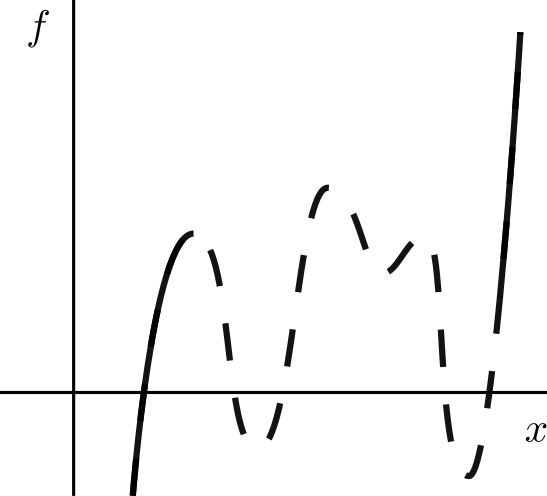
\includegraphics[width=\tttp]{../Pictures/Odd_poly.png}}
\subfigure[\label{Even_polynomial}]{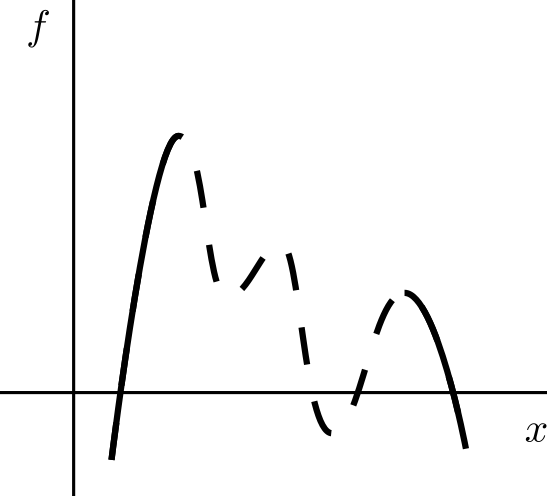
\includegraphics[width=\tttp]{../Pictures/Even_poly.png}}\\
\caption{\label{Poly_sketches}Basic polynomial properties. The lines have dashed centres as the shape can be altered depending on the specific polynomial used. However, the minimum number of roots can be guaranteed (if there are any). (a) A general odd polynomial. (b) A general even polynomial (with negative leading order term).}
\end{figure}



\subsubsection{Hill functions}
Hill functions are also common functions that are used widely as they can cover a wide variety of outcomes. They have the form
\bb
f(x)=\frac{\alpha x^m}{\beta^n+x^n},\label{Hill_function}
\ee
where $\alpha$ and $\beta$ are control parameters.

Although, below, we consider $\alpha=\beta=1$ changing these parameters does not, generally, change the qualitative properties we are illustrating. The parameters, only tend to influence the quantitative behaviour of the function \eg how big the gradients are, or where the transitions happen. 

Generally, $m=n$ (which is the usual definition of the Hill function), but there is no reason why this is so. Further, the function has different properties for the different cases of $m$ relative to $n$. See \fig{Hill_functions} for the possible outcomes. In all cases the dynamics will be dominated by $x^m$ for small $x$ and $x^{m-n}$ for large $x$. This is why we need to consider the sign of $m-n$.
\begin{itemize}
\item When $m>n$, although there maybe stationary points, the curve will eventually tend to grow without bound.
\item When $m=n$, $x^{m-n}=1$. Thus, the function asymptotes to $f\rightarrow 1$. Such Hill functions are used as ``switches'', namely one type of dynamic occurs when $x$ is small and another occurs when $x$ is large. Steepness of the switch is controlled by the size of $m=n$; larger values create a sharper transition.
\item When $m<n$, $x^{m-n}=1/x^{n-m}\rightarrow 0$ as $x\rightarrow 0$. Thus, although we have an initial hump the curve decays to zero.
\end{itemize}
Thus, we can see why Hill functions are so powerful, namely, they are able to describe growth, saturation and decay all through the sign of $m-n$.


\begin{figure}[p!!!h!!!tbp]
\centering
\subfigure[\label{Hill_m>n}$m>n$]{\includegraphics[width=\tttp]{../Pictures/mn1.png}}
\subfigure[\label{Hill_m=n}$m=n$]{\includegraphics[width=\tttp]{../Pictures/mn2.png}}
\subfigure[\label{Hill_m<n}$m<n$]{\includegraphics[width=\tttp]{../Pictures/mn3.png}}
\caption{\label{Hill_functions} The general shape of Hill functions, \eqn{Hill_function}, with (a) $m>n$, (b) $m=n$ and (c) $m<n$.}
\end{figure}

\section{Phase planes}
\subsection{One-dimensional}\label{One-dimensional}
In one dimension the phase plane is a plot of the dynamics in the $(u,\dot{u})$ plane. Steady states can easily be read off as they are where the curve crosses the $x$-axis. Equally, we can determine the stability of the steady states by considering where the curve lies.

Specifically, if whenever the curve lies in the top half plane $\dot{u}>0$ and, thus, $u$ increases over time. Thus, $u$ will increase without bound, or until the curve crosses the $x$-axis, at which point $\dot{x}=0$. Similarly, in the bottom half plane $\dot{u}<0$ and, so, $u$ decreases over time, either without bound, or until the curve cuts the $x$-axis.

\begin{example}[frametitle=Logistic equation phase plane\label{Logistic_equation_phase_plane}]
Consider
\bb
\dot{u}=u(1-u).
\ee
\COL{The phase plane of the logistic equation is plotted with dynamic arrows in \fig{Logistic_phase_plane}. Critically, these arrows verify the results seen in example \ref{Logistic_stability_example}, namely, $u=0$ is unstable as trajectories diverge away from it, whilst $u=1$ is stable as trajectories tend to this state. These insights match those gained from example \ref{Logistic_stability_example}.
}
\end{example}
\begin{figure}[!!!h!!!tb]
\centering
\includegraphics[width=\ttp]{../Pictures/Logistic_stability.png}
\caption{ \label{Logistic_phase_plane} The phase plane plot of the logistic curve in $(u,\dot{u})$ coordinates.}
\end{figure}

\subsection{Two-dimensional}
In \sect{One-dimensional} we could understand the entire dynamics of a one species system in the $(u,\dot{u})$ plane. We would like to gain the same information for systems with multiple populations However, when we have two variables we would have to plot four variable $(u,v,\dot{u},\dot{v})$, which is hard to visualise and almost impossible to sketch. Thus, we simplify our plot and only consider the $(u,v)$ plane instead, which is known as the `phase plane'. To construct a phase plane (instead of considering a single trajectory, as in the $(t,u)$ simulation) we consider the motion of a trajectory across all points in the $(u,v)$ space.

To aid in our understanding we introduce a new concept. 
\begin{defin}
Consider an ODE system
\bb
\dot{\bm{u}}=\bm{F}(\bm{u}),
\ee
where $\bm{F}(\bm{u})=(F_1(u_1,\dots,u_n),\dots,F_n(u_1,\dots,u_n))$. The nullclines are the curves defined by
\bb
F_i(u_1,\dots,u_n)=0,
\ee
for all $i=1,\dots,n$.
\end{defin}
Nullclines are a useful concept because on each separate curve the dynamics of at least one variable is stationary, thus, the direction across a nullcline is simplified. Moreover, if all nullclines meet at a given point all dynamics must be stationary, \ie by definition all nullclines meet at steady states.

The nullclines then delineate different dynamical regions. Namely, consider a general nullcline, for example $\dot{u}=0$, on one side of the line $\dot{u}>0$, whilst on the other $\dot{u}<0$ (not this is not necessarily true). The same can be said of the $\dot{v}=0$. Thus, the nullclines segment the $(u,v)$ into regions of different dynamics. With this knowledge we can specify the signs of the derivatives in each region and, thus, sketch what will happen in each case.

\begin{example}[frametitle=Two-dimensional phase plane]\label{Nullcline_example_example}
Consider the system
\begin{align}
\dot{u}&=v-(u-2)(u-3),\label{Nullcline_1}\\
\dot{v}&=v-\ln(u),\label{Nullcline_2}
\end{align}
in the half plane $u>0$.

\COL{The steady states of this would satisfy
\bb
\ln(u)=(u-2)(u-3),
\ee
which has no closed form solution. We could estimate the solutions using a numerical root finding }\COL{algorithm. However, by plotting the nullclines,
\begin{align}
v&=(u-2)(u-3),\\
v&=\ln(u),
\end{align}
in \fig{Nullcline_example}, we immediately  see there are exactly two steady states.}

\COL{We first consider the $\dot{u}$ nullcline
\bb
v=(u-2)(u-3),
\ee}
\COL{illustrated in \fig{u_nullcline}. Pick any point vertically higher than the curve, \eg (2,10), and consider the sign of \eqn{Nullcline_1}. Specifically, substituting this value in we get
\bb
\dot{u}=10>0.
\ee
Thus, above the curve $\dot{u}>0$ and $\dot{u}<0$ below the curve \see{u_nullcline}. Once, we know the sign of the derivative in each section we can draw arrows to illustrate the local direction in which the trajectory will be heading. For example, in a region with $\dot{u}>0$ the $u$ coordinate will be increasing and, so the arrowhead points to the right \ie increasing $u$ direction.

We can do the same for the $v$ regions. For example, consider the point $(5,0)$,
\bb
\dot{v}=0-\ln(5)<0.
\ee
Hence, to the right of the $v$ nullcline $v$ is decreasing. By a similar process $v$ is increasing to the left of the $v$ nullcline \see{v_nullcline}.

We now combine this information in each region providing a sketch of how a trajectory will act anywhere in the plane. In addition we add arrows the nullclines where we remember that there is no movement in the $u$ direction on the $u$ nullcline and no movement in the $v$ direction along the $v$ nullcline. Namely, the arrows are vertical and horizontal on the $u$ and $v$ nullclines, respectively. Equally, we pay explicit attention to which way these arrows are directed according to the surrounding information.

All of this information is plotted in \fig{uv_nullcline}. Critically, in this case we are able to suggest what forms the steady states will have. The steady state on the left (approximately (1.6,0.5)) will be unstable because all of the arrows near to the steady state point away from the steady state. The steady state on the right (approximately, (3.8,1.3)) appears to be a saddle as arrows in the horizontal direction point towards the steady state, whilst arrows in the vertical direction point away from the state.

However, to ensure we are right we have to run the analysis. We will not do this here because the algebra gets very hairy and, as mentioned, you would need to use a numerical root finder to estimate the steady states to substitute into the Jacobian. If we do do this numerically we find that the eigenvalues of the left steady state are $\lambda_\pm\approx 1.36\pm0.69I$, thus, the point is indeed unstable, but an unstable spiral, which we could not have predicted from the graph. The eigenvalues for the steady state on the right are $\lambda_-\approx -2.43<0<0.92=\lambda_+$, hence the point is a saddle, justifying our diagram.}
\end{example}



From this example we have seen that phase planes are helpful diagrams, which encapsulate lots of stability information. However, as illustrated, in comparing the diagram with the actual analytical values of the eigenvalues it can be difficult to tell the difference between (un)stable nodes and (un)stable spirals. Equally, sketches only provide the correct insight if you draw the system correctly. If there had been a parameter in this system that we could vary then there may have been a stability case, dependent on the parameter, that we would miss if we had only drawn one diagram. Thus, a phase plane should always be backed up with linear analysis. The linear analysis provides the local information, whilst the phase plane allows us to approximately see how all the dynamics fit together.

\begin{figure}[p!!!h!!!tbp]
\centering
\subfigure[\label{Nullcline_example}]{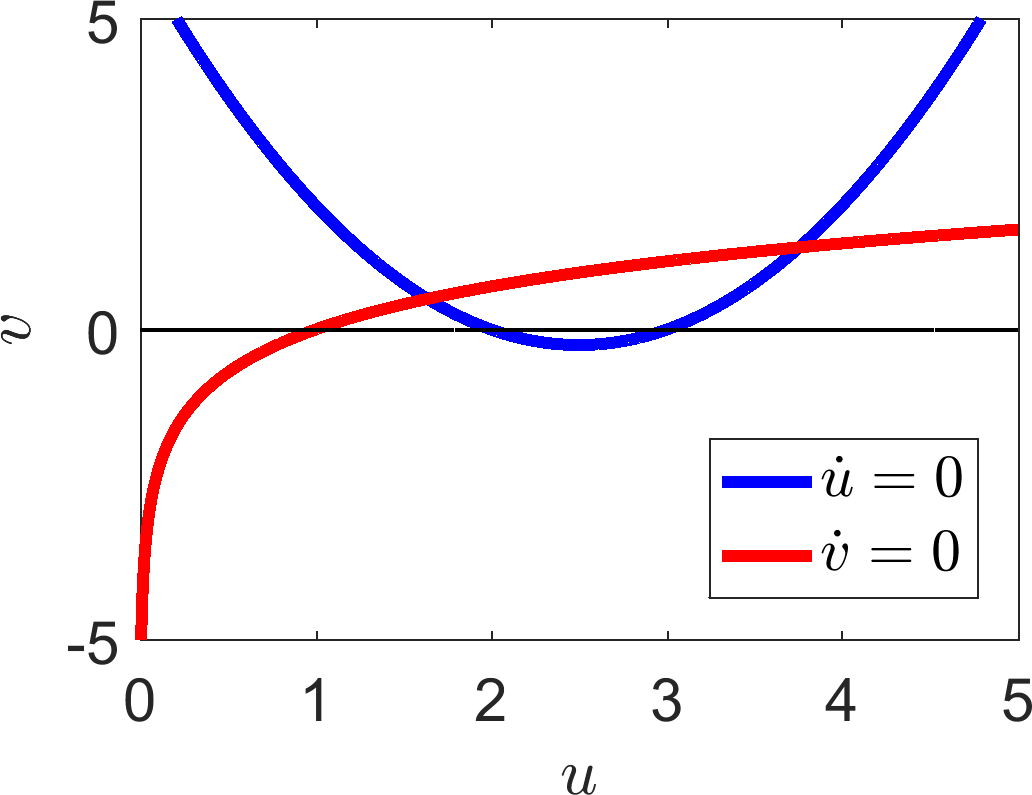
\includegraphics[width=\ttp]{../Pictures/Nullcline_example.png}}\\
\subfigure[\label{u_nullcline}]{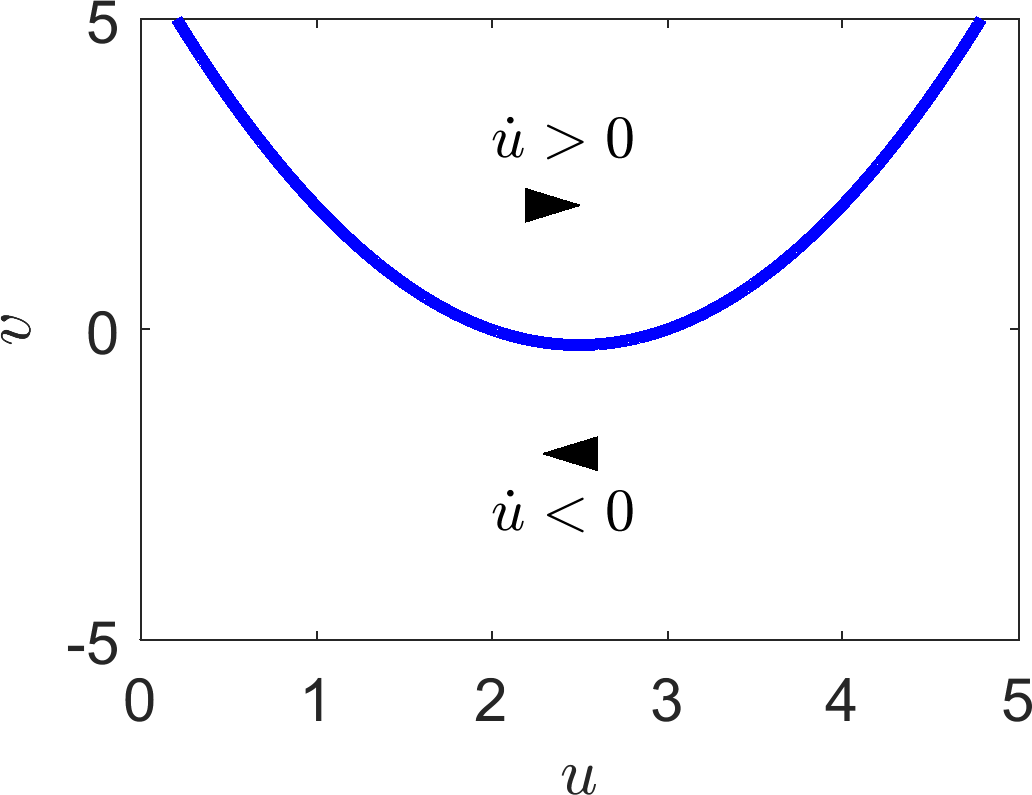
\includegraphics[width=\ttp]{../Pictures/u_nullcline.png}}
\subfigure[\label{v_nullcline}]{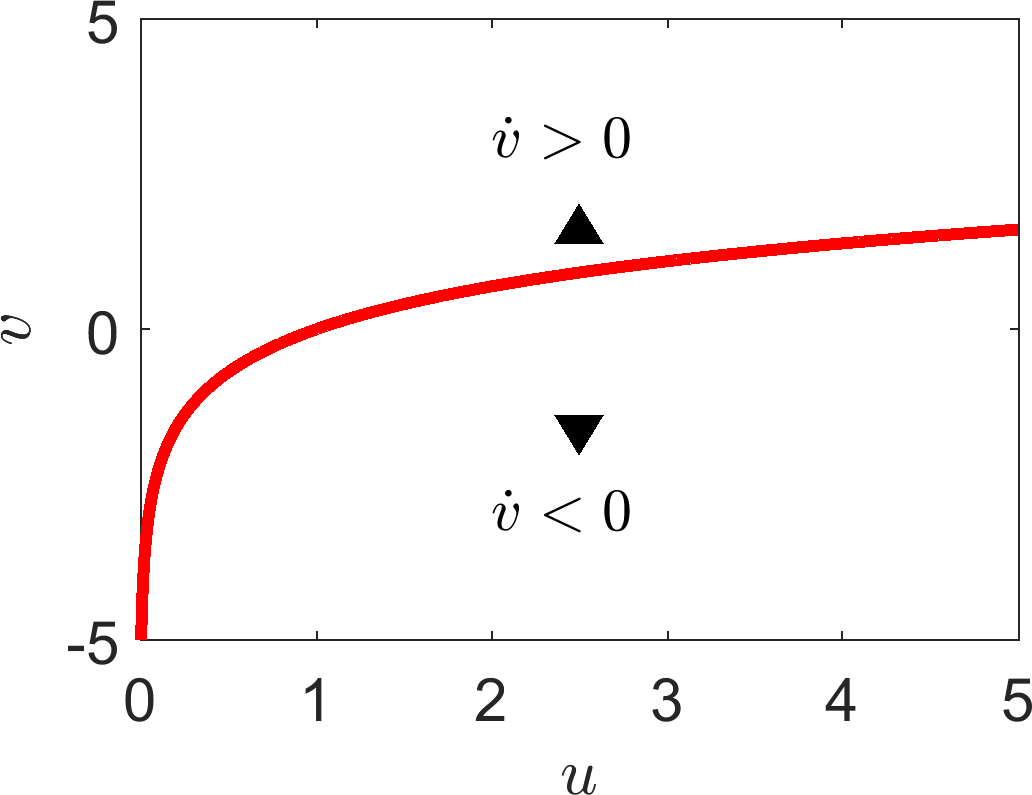
\includegraphics[width=\ttp]{../Pictures/v_nullcline.png}}
\subfigure[\label{uv_nullcline}]{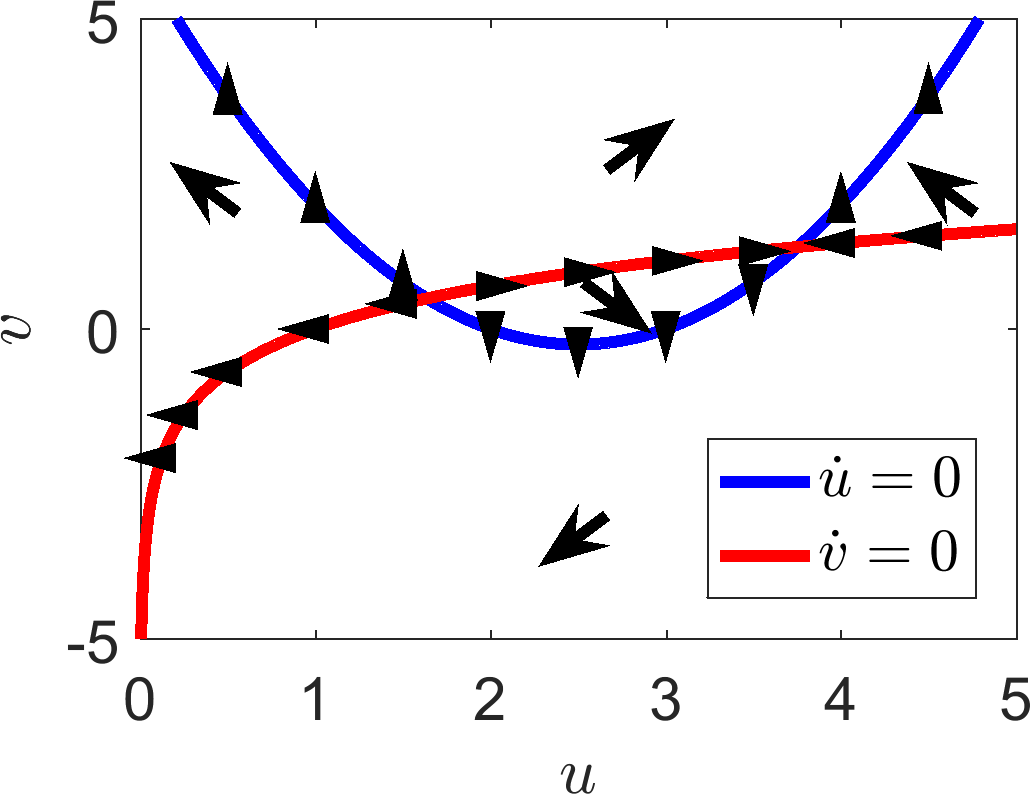
\includegraphics[width=\ttp]{../Pictures/uv_nullcline.png}}
\subfigure[\label{Phase_plane_example}]{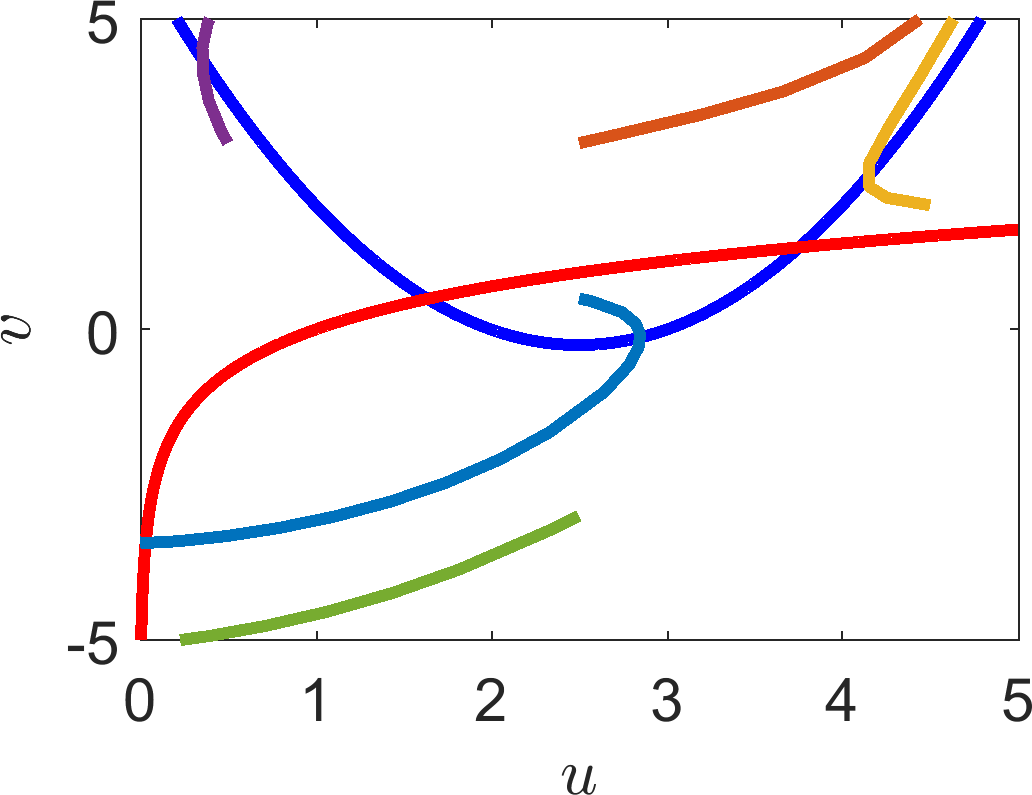
\includegraphics[width=\ttp]{../Pictures/Phase_plane_example.png}}
\caption{\label{Derivative_signs}(a) Plot of the nullclines of \eqns{Nullcline_1}{Nullcline_2}. Specifying the signs of the derivatives on either side of the (b) $\dot{u}$ and (c) $\dot{v}$ nullcline. The arrowheads indicate the general direction that a trajectory will be heading. These results can then be combined into the direction plots seen in (d). Finally, in (e), we simulate a number of trajectories, which demonstrate that the arrows in (d) provide the correct general idea.}
\end{figure}


\section{Check list}
By the end of this chapter you should be able to:
\begin{todolist}
\item reproduce all definitions;
\item convert a system of population interactions into reaction equations;
\item convert reaction equations into ODEs using the Law of Mass Action;
\item non-dimensionalise a system of equations using direct substitution, or the arrow method;
\item sketch simple curves
\item derive the steady states and their dependence on any given parameters;
\item derive the stability of the  steady states and their dependence on any given parameters;
\item identify parameter dependent bifurcations;
\item define what a nullcline is;
\item understand the relationship between steady states and the points at which nullclines cross;
\item plot nullclines;
\item sketch arrows showing general trajectory directions on the phase plane;
\item interpret the stability of the steady states from the information plotted on a phase plane.
\end{todolist}
